\chapter{针对形变的理论建模}

\section{使用数据}
使用上一章得到的平均形变速率作为建模的输入数据,
对于该区域中部的明显形变采用Mogi模型建模。

\section{Mogi模型}
Mogi模型\cite{mogiRelationsEruptionsVarious1958}是
日本学者Mogi于1958年提出来的理论模型。
Mogi模型根据理论公式建立了扰动源的参数和地表形变之间的关系,
在火山领域有很广泛的应用
\cite{luSatelliteRadarInterferometry1998,luSyntheticApertureRadar2000,
luMagmaticInflationDormant2002,luInterferometricSyntheticAperture2005,
luGroundSurfaceDeformation2010}。
后来随着InSAR技术应用的范围增大,
Mogi模型也应用于地下水的抽取与注入\cite{zhengWastewaterLeakageWest2019}。

它的基本假设为:
\begin{enumerate}
    \item 介质为各项同性线性弹性介质,可以用剪切模量$\mu$和泊松比$\nu$完全表征介质的特性。
    \item 研究空间为半空间。
    \item 扰动源为点源,即源的尺度远小于模型的尺度:$\alpha \ll d$。
\end{enumerate}

根据基本假设,由连续介质力学的基本理论可以推导:
\begin{equation}
    \left(\begin{array}{c}
        u \\ v \\ w \\
    \end{array}\right)
    =\frac{\Delta V(1-\nu)}{\pi R^3}
    \left(\begin{array}{c}
        x \\ y \\ d \\
    \end{array}\right)
    \label{eq:mogi}
\end{equation}
其中点源的坐标为$(0,0,-d)$,$(x,y,0)$为地表某一点,$(u,v,w)$为该点的位移,
$R$为扰动源到地面一点的距离,有
\begin{equation}
    R^2=x^2+y^2+d^2
\end{equation}

由以上基本假设可以得知,Mogi模型的参数分为两个部分:
\begin{enumerate}
    \item 扰动源的参数:扰动源的位置$X,Y,Z$,以及表征扰动大小的体积变化$DV$。
    \item 介质的参数:泊松比$\nu$。
\end{enumerate}
注意公式\ref{eq:mogi}中不含剪切模量$\mu$,这完全是由Mogi模型的特殊性造成的。
地球实际介质泊松比$\nu$波动不大,对反演的结果影响不大,一般设成已知量。
主要的反演参数为扰动源的四个参数。

\section{反演过程和结果}
本研究使用的建模软件为GBIS,关于反演算法和软件已经在第\ref{ch:pm}章中说明。
为了节省运算时间,首先对数据进行quadtree重采样,
设置quadtree重采样的标准差阈值为$\rm 10^{-5}m$。
采样前后的对比如图\ref{fig:unsample}和\ref{fig:subsample}所示。
\begin{figure}[htp]
    \centering
    \begin{minipage}{0.85\textwidth}
        \centering
        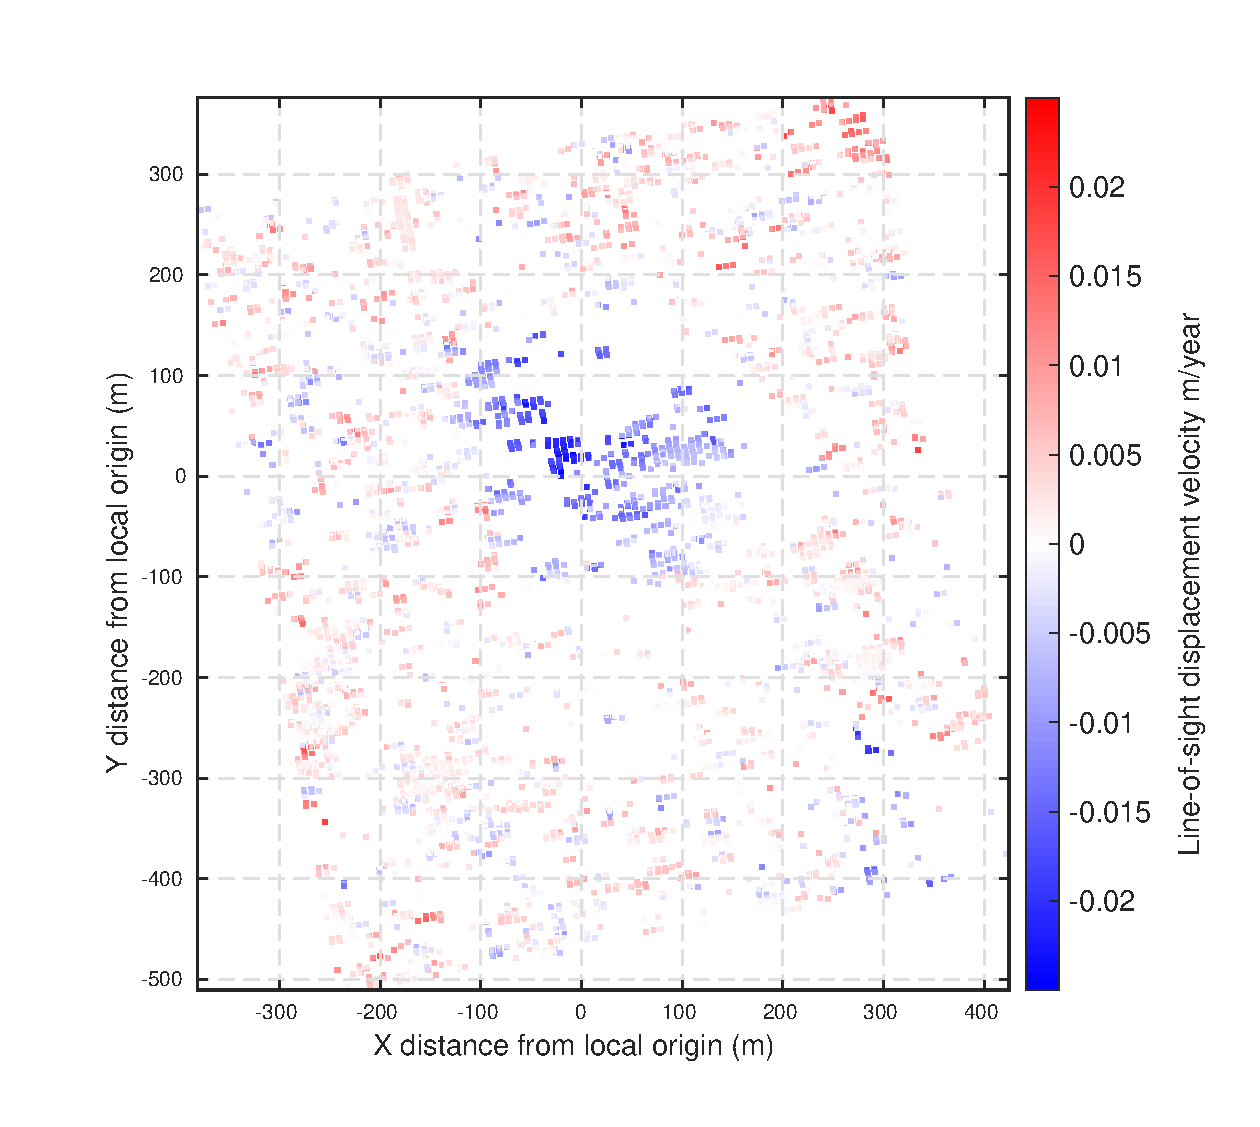
\includegraphics[width=\textwidth]{unwrapped.eps}
        \caption{原始形变图}
        \label{fig:unsample}
    \end{minipage}
    \qquad
    \begin{minipage}{0.85\textwidth}
        \centering
        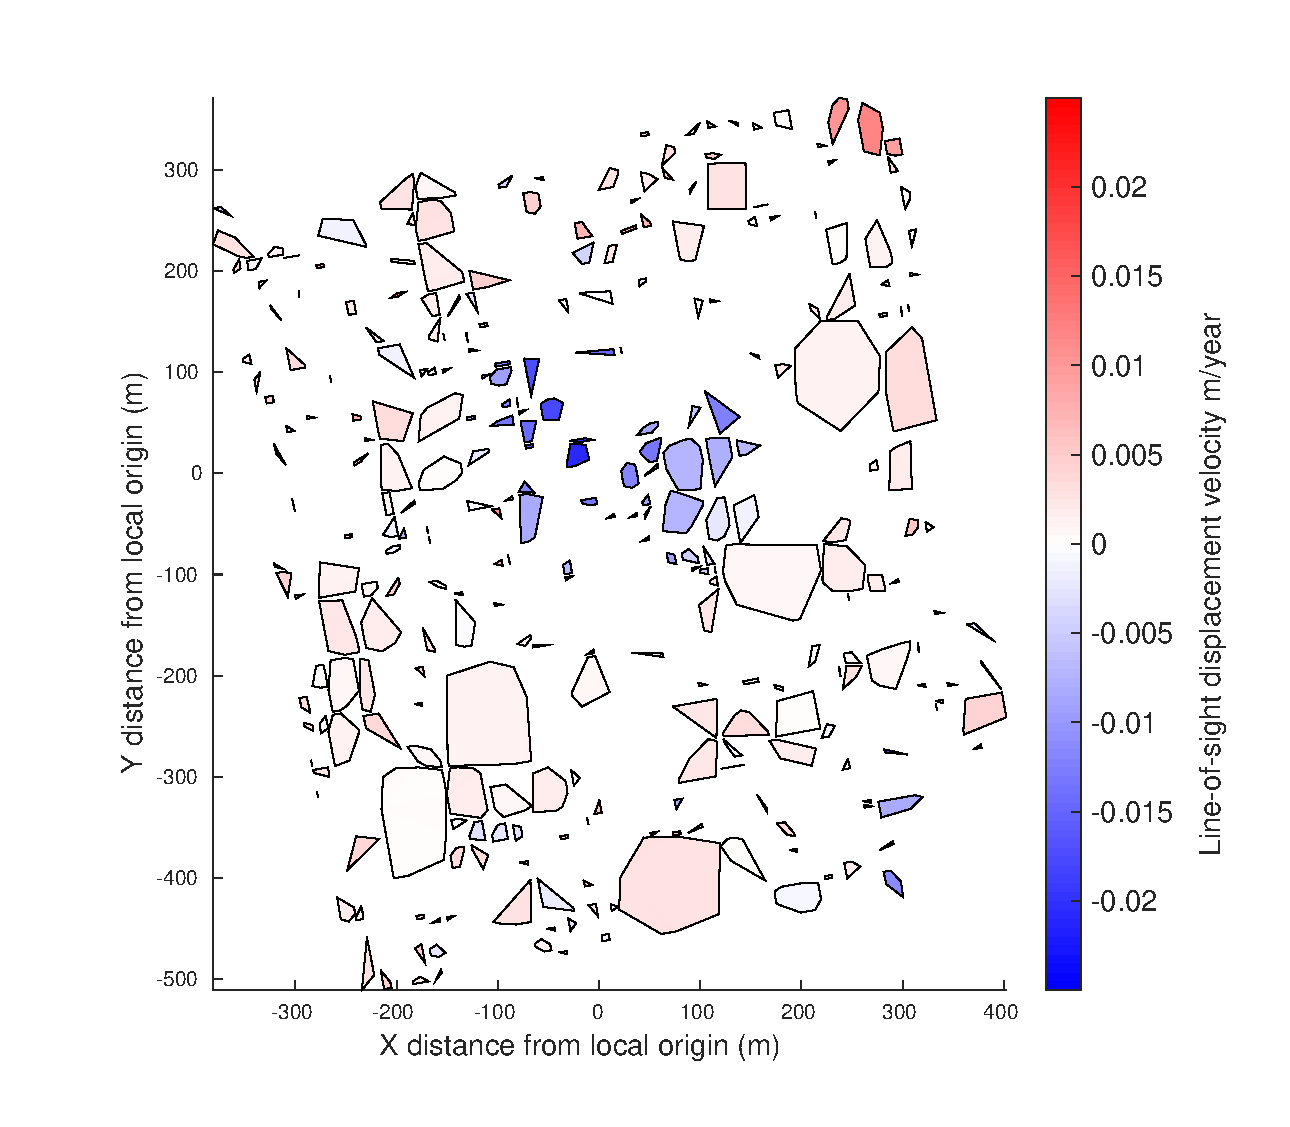
\includegraphics[width=\textwidth]{subsampled.eps}
        \caption{quadtree采样后的形变图}
        \label{fig:subsample}
    \end{minipage}
\end{figure}
然后开始反演。反演的结果见表\ref{tab:modelpar}。
\begin{table}[htb]
    \centering\small
    \caption{模型参数}
    \label{tab:modelpar}
    \begin{tabular}{@{}cccccc@{}}
    \toprule
    参数       & 最优值 & 平均值 & 中位值 & 2.5\% & 97.5\% \\ 
    \midrule
    Mogi X/m    & -11.7061 & -12.1911 & -12.0754 & -30.0636 & 5.79259\\
    Mogi Y/m     & 45.2833 & 45.9855 & 46.1422 & 24.6177 & 66.6009\\
    Mogi depth/m & 104.739 & 108.746 & 107.288 & 86.7258 & 135.813\\
    Mogi DV/$\rm m^3$   & -1137.49 & -1173.04 & -1149.94 & -1647.73 & -793.301\\
    InSAR 常数 & 0.00219907	& 0.00217916 & 0.00216868 & 0.00116873 & 0.00322181\\
    \bottomrule
    \end{tabular}
\end{table}
参数的后验概率见图\ref{fig:pdf}。
从该图中可以看出,四个参数的收敛性都比较好。
\begin{figure}[htb]
    \centering
    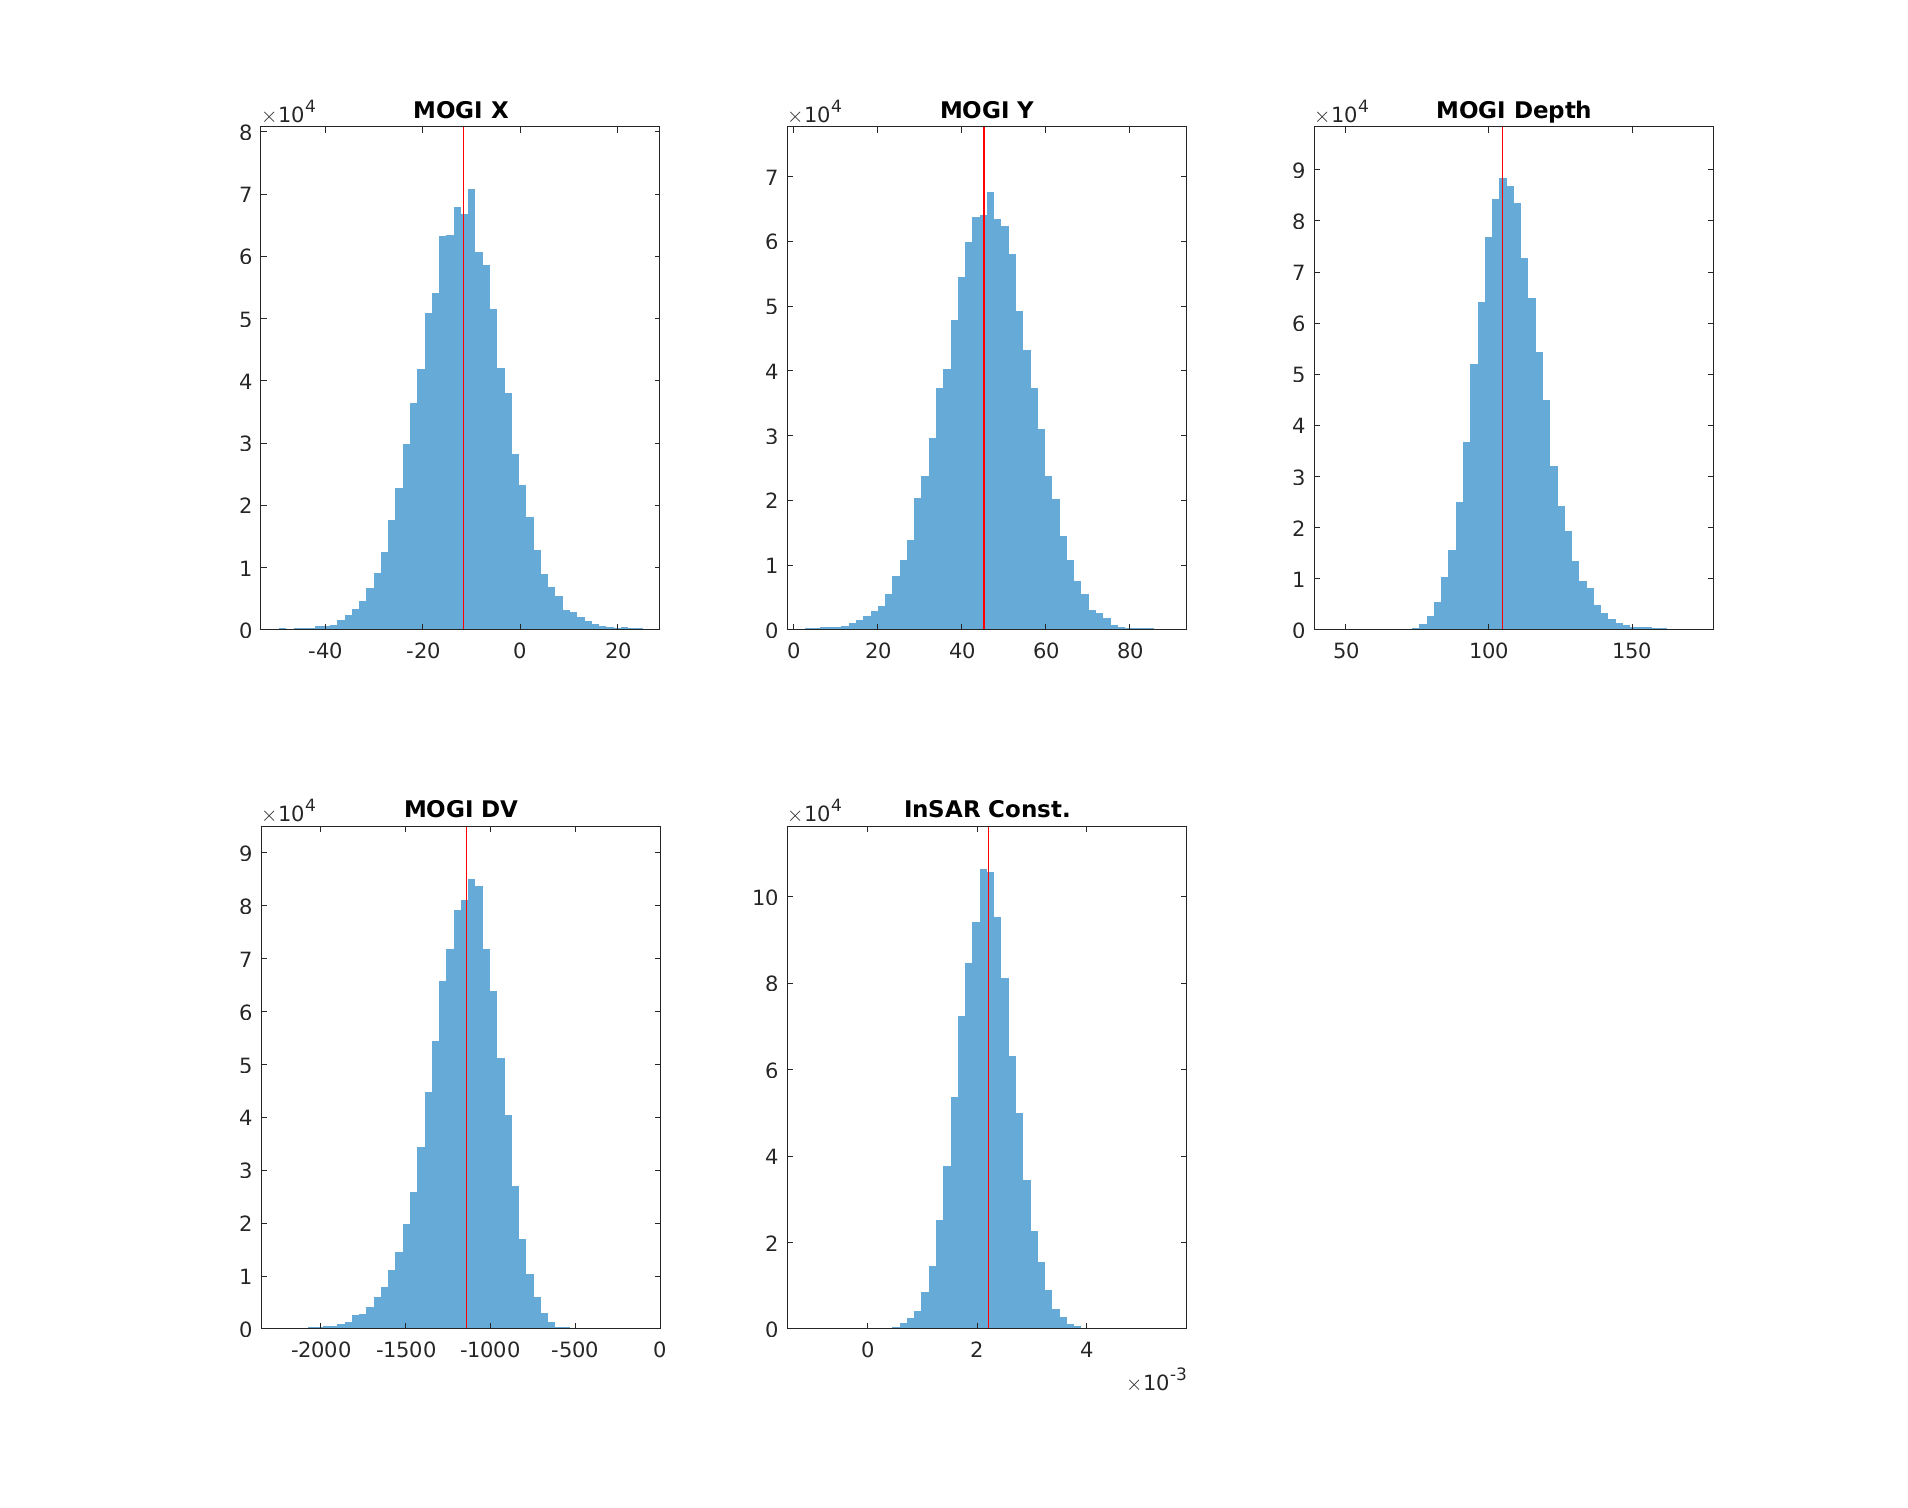
\includegraphics[width=1.0\textwidth]{PDFs.eps}
    \caption{反演参数的后验概率分布}
    \label{fig:pdf}
\end{figure}
原始形变数据,反演参数理论行便和二者的差见图\ref{fig:residual}。

从图\ref{fig:residual}来看,反演比较成功,模型反推的结果和InSAR观测的结果吻合得比较好。
但从图中可以看出,InSAR的结果仍有很多不吻合的地方。
一方面,可能是数据处理的原因,本研究分析的区域较小,大概在1平方公里左右,
所得到的PS点也不够密集,不一定能比较全面地覆盖当地的所有形变特征。
另一方面,也有可能是模型较为粗糙的原因,Mogi模型是比较简单的模型,
可能实际导致形变的扰动源比较复杂。
从图\ref{fig:residual}中的剩余形变图可以看出,该区域的下半部分有不太明显的下沉,上半部分有一定的上升,
这部分的形变没有被Mogi模型解释,如果采用更精确的模型,可能会有更好的反演效果。

\section{与其他研究成果的比较}
由于本研究的研究区域在Carlsbad市区,和两条重要的高速公路相邻,一旦坍塌会造成相当大的损失。
所以,当地政府组织相关专业人员对此地进行了详尽的调查。

2009年,某一二维地震反射评估给出了该卤水井内部的空洞的大概形状。
空洞的中心在尤金妮娅1号钻井处,近似呈梨型,北部较窄,南部较宽。
2011年又开展了该处高分辨率大地电磁调查\cite{landElectricalResistivitySurvey2011},研究发现此区域地下有较明显的低阻区。
低阻区向北延伸至285和62-180两条高速公路,向南延伸至CID南方运河。
这是该区域地下空洞的有效证明。
此后,当地相关部门和公司通过诸多手段得到了地下空洞的详细分布,并于2018年9月展开空洞填补工作。
从有关部门给出的地下空洞的详细信息来看,本研究所建的模型中扰动源的X,Y位置比较精确,
但深度差距比较大,模型中深度为地下103m,但实际的空洞在140m到180m之间。
深入差距比较大的原因应该是所用的Mogi模型导致形变和实际空洞导致形变的物理原理上有一定的差异,
如果采用更准确的空洞模型应该会有更好的反演结果。

比较以上工作和InSAR的成果,可以得到以下结论。
\begin{enumerate}
    \item InSAR在此类问题中能起到一定的作用,InSAR能比较精确地估计出沉降区域的位置和大小;
    \item InSAR和地震,大地电磁方法相比,要节约很大的成本;
    \item InSAR能得到地表的变形数据,在坍塌预测方面有不可替代的作用;
    \item 和地震,大地电磁方法相比,InSAR方法无法得到精确的空洞形状等信息。
\end{enumerate}

\begin{landscape}
\begin{figure}[htb]
    \centering
    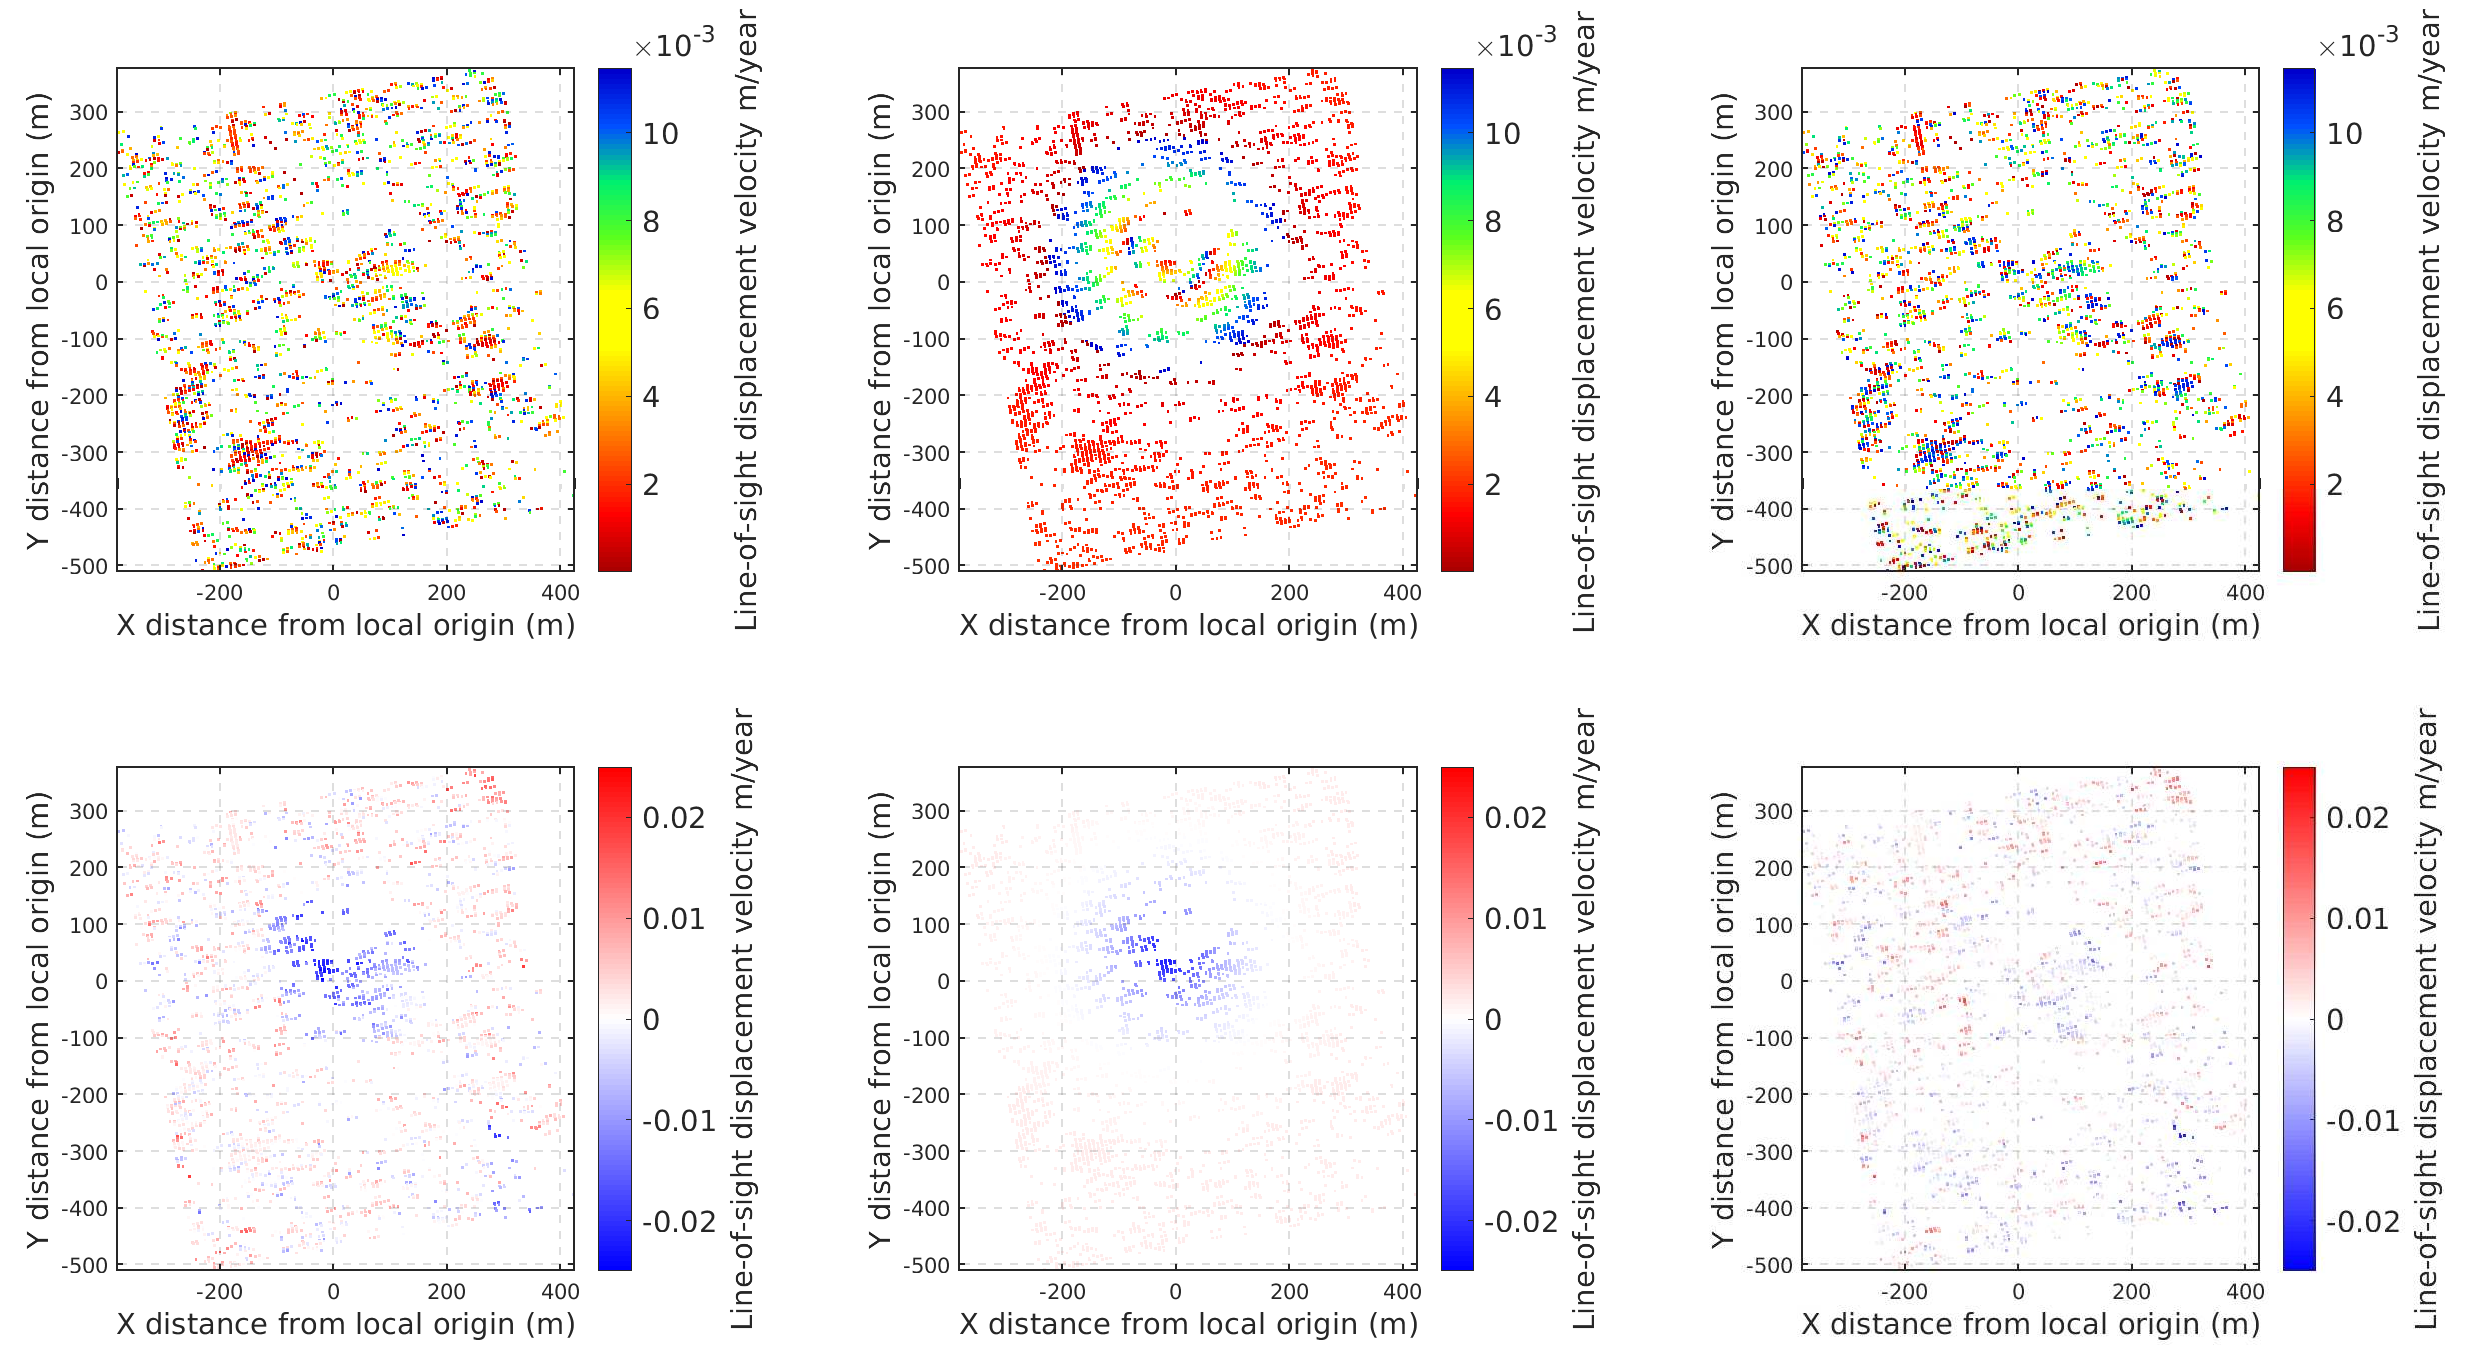
\includegraphics[width=1.5\textwidth]{croppedResidual.pdf}
    \caption{原始形变数据,反演参数理论形变以及二者的差}
    \note{注:六副图中,上面三副为未解缠的数据,下面三副为解缠之后的数据;
    左边的图为原始形变的数据,中间的图为模型理论推导的形变数据,右边为原始数据减去理论数据的剩余数据。}
    \label{fig:residual}
\end{figure}
\end{landscape}